\chapter{Azure DevOps}


\section{About Azure DevOps Enterprise \& Cloud}

Azure DevOps Enterprise is an on-premise variation of the cloud-hosted Azure DevOps services.
Both versions are compatible with \cxoneflow and are generically referred to Azure DevOps Enterprise
throughout this documentation.

The \cxoneflow endpoint \texttt{/adoe} is the handler for all webhook event
payloads originating from Azure DevOps Enterprise.  

\section{Webhook Topology}

Azure DevOps Enterprise (on-premise) uses one or more \textbf{Collection} logical units to separate
repositories into logical groups.  A \textbf{Collection} in Azure DevOps Enterprise 
corresponds to a Azure DevOps Cloud \textbf{Organization} in that the \textbf{Organization} is a logical unit 
that separates repositories into logical groups. Web hook deployments are not available at this scope.

In each \textbf{Collection} or \textbf{Organization}, zero or more \textbf{Project} logical
units establish the next level of repository organization.  Each \textbf{Project} will 
have one or more \textbf{Repository} units that will contain code that should be scanned.  Webhooks
can be deployed at this scope; each \textbf{Repository} in the configured \textbf{Project} logical unit
will emit webhook events when Service Hooks have been configured in the \textbf{Project} to
deliver webhook events to \cxoneflow.

Configuration of Service Hooks at the \textbf{Project} scope is generally the preferred
method of webhook deployment for Azure DevOps.

Webhooks can be deployed at the scope of each \textbf{Repository} if desired.  The number of repositories
in a large enterprise generally makes deployment at the \textbf{Repository} scope useful
only for testing purposes.



\section{Webhook Configuration}

Webhook configurations applied at the \textbf{Project} scope are ideal given
that this configuration delivers webhook events to \cxoneflow for all repositories in the project.
The project name will appear in clone URLs and can be used as part of the regular expression configured
for the \texttt{repo-match} configuration element.  Please see Section \ref{sec:yaml-config} for a description
of the \texttt{repo-match} configuration element.

The project's "Service Hooks" can be used to configure webhook events to be delivered to the
\cxoneflow \texttt{/adoe} endpoint for each repository in the organization.  Azure DevOps
Enterprise will require multiple service hook definitions to handle different classes
of repository events.

Figure \ref{fig:adoe-hook-config} shows the initial service hook configuration with the 
"Web Hooks" option selected.  Clicking the \textbf{Next} button will display the 
event trigger configuration as depicted in Figure \ref{fig:adoe-trigger-config}. 
The trigger type of event for \textbf{Code pushed} should be selected.
Clicking the \textbf{Next} button will display the \textbf{Action} configuration
where the webhook connection parameters can be configured.

Figure \ref{fig:adoe-endpoint-config} shows the configuration where the \cxoneflow
endpoint connection configuration is to be provided.  A URL with the suffix
\texttt{/adoe} and the \textit{Basic authentication password} is the only
field that is required by \cxoneflow\footnote{Azure DevOps Enterprise will require
the use of an encrypted endpoint when using the basic authorization password.}.
The basic authentication password should match the \texttt{shared-secret} \cxoneflow
configuration element.  Please see section \ref{sec:yaml-config}
for more information about the \texttt{shared-secret} configuration.

The \textbf{Test} button can be used to validate connectivity to the \cxoneflow endpoint.
The secret is not currently part of the connectivity validation; if the \cxoneflow logs
are showing messages indicating webhook events are being rejected, checking that the
shared secret matches in both the Azure DevOps Enterprise service hook and \cxoneflow
configurations.

A complete configuration should emit web hook payloads on the following events:

\begin{itemize}
    \item Code pushed
    \item Pull request created
    \item Pull request updated
\end{itemize}

\begin{figure}[ht]
    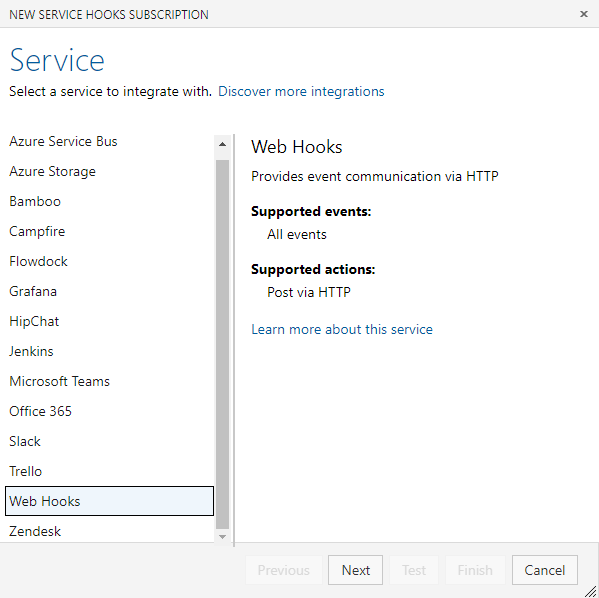
\includegraphics[width=\textwidth]{graphics/adoe-service-hooks-sub.png}
    \caption{Azure DevOps Enterprise Service Hook Configuration}
    \label{fig:adoe-hook-config}
\end{figure}

\begin{figure}[ht]
    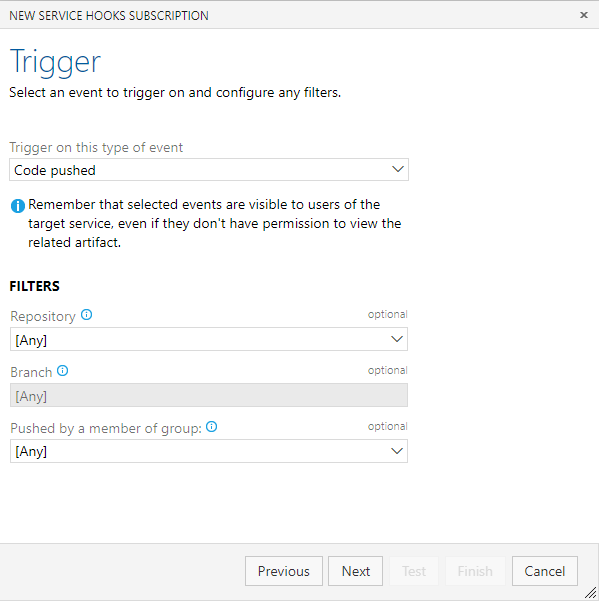
\includegraphics[width=\textwidth]{graphics/adoe-hook-trigger-config.png}
    \caption{Azure DevOps Enterprise Web Hook Trigger Configuration}
    \label{fig:adoe-trigger-config}
\end{figure}

\begin{figure}[ht]
    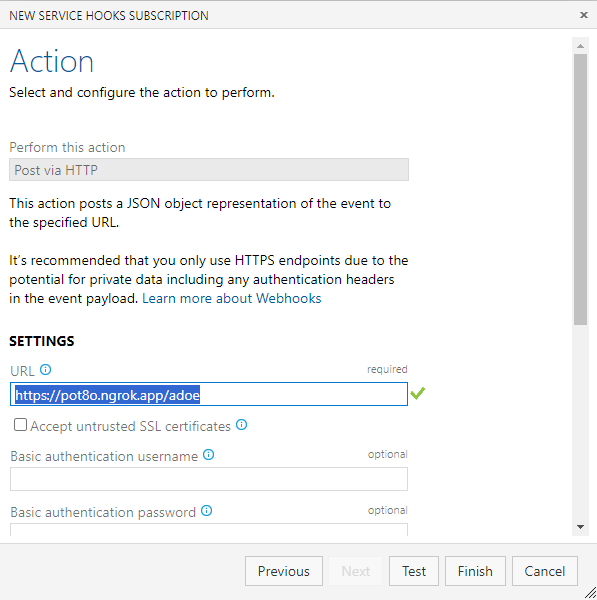
\includegraphics[width=\textwidth]{graphics/adoe-hook-endpoint-config.png}
    \caption{Azure DevOps Enterprise Web Hook Endpoint Configuration}
    \label{fig:adoe-endpoint-config}
\end{figure}

\section{\cxoneflowtext\space Service Account}

Azure DevOps Enterprise utilizes user accounts to define access.  \cxoneflow will require
at least one user account to use as a service account for API and cloning operations.  The
service account must be in the \textit{Contributor} group for each project for which
that account will orchestrate scans.  It is possible to create a single service account that
is used for all projects if the service account is assigned as a contributor to all
relevant projects.  The \cxoneflow configuration can accommodate multiple user accounts
if there is a need to have separate service accounts for some projects.

\section{\cxoneflowtext\space SSH Keys}

While performing scan orchestration, \cxoneflow does access the Azure DevOps Enterprise API for
certain operations.  This requires a configuration in the \texttt{api-auth} configuration
element as described in Section \ref{sec:yaml-config}.  The \texttt{clone-auth} element,
described in Section \ref{sec:yaml-config}, is an optional element where the credentials
used for cloning code can be provided.  If \texttt{clone-auth} is not provided, cloning will
be attempted using the credentials defined by \texttt{api-auth}.

The \texttt{clone-auth} configuration can define an SSH private key for use in cloning.  This
will allow for a separate set of credentials or authentication methods between cloning and
API use.

\section{Protected Branches}

Each repository in Azure DevOps Enterprise has a default branch defined in the project
configuration.  The repository's default branch is considered the protected branch for
workflow logic purposes.  Any push to the default branch or pull request that targets
the default branch will cause \cxoneflow to orchestrate a scan.
